\documentclass{article}

\usepackage{graphics}
\usepackage{tikz}
\pgfrealjobname{ordering}
\usetikzlibrary{arrows}

\begin{document}

\beginpgfgraphicnamed{ordering-tikz}
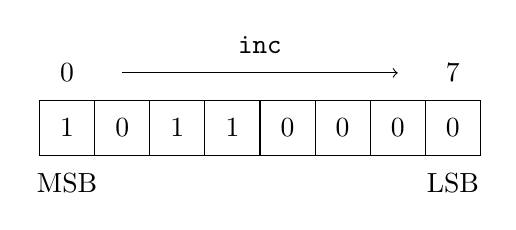
\begin{tikzpicture}[scale=0.7]
  \draw (0,0) rectangle (1,1) node[pos=.5] {1};
  \draw (1,0) rectangle (2,1) node[pos=.5] {0};
  \draw (2,0) rectangle (3,1) node[pos=.5] {1};
  \draw (3,0) rectangle (4,1) node[pos=.5] {1};
  \draw (4,0) rectangle (5,1) node[pos=.5] {0};
  \draw (5,0) rectangle (6,1) node[pos=.5] {0};
  \draw (6,0) rectangle (7,1) node[pos=.5] {0};
  \draw (7,0) rectangle (8,1) node[pos=.5] {0};

  \node at (.5,1.5) {0};
  \node at (7.5,1.5) {7};
  \draw[->] (1.5,1.5) -- (6.5,1.5);
  \node at (.5,-0.5) {MSB};
  \node at (7.5,-0.5) {LSB};
  \node at (4,2) {\texttt{inc}};
\end{tikzpicture}
\qquad
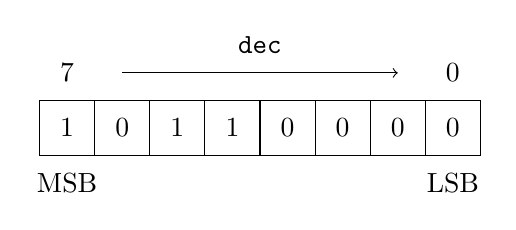
\begin{tikzpicture}[scale=0.7]
  \draw (0,0) rectangle (1,1) node[pos=.5] {1};
  \draw (1,0) rectangle (2,1) node[pos=.5] {0};
  \draw (2,0) rectangle (3,1) node[pos=.5] {1};
  \draw (3,0) rectangle (4,1) node[pos=.5] {1};
  \draw (4,0) rectangle (5,1) node[pos=.5] {0};
  \draw (5,0) rectangle (6,1) node[pos=.5] {0};
  \draw (6,0) rectangle (7,1) node[pos=.5] {0};
  \draw (7,0) rectangle (8,1) node[pos=.5] {0};

  \node at (.5,1.5) {7};
  \node at (7.5,1.5) {0};
  \draw[->] (1.5,1.5) -- (6.5,1.5);
  \node at (.5,-0.5) {MSB};
  \node at (7.5,-0.5) {LSB};
  \node at (4,2) {\texttt{dec}};
\end{tikzpicture}
\endpgfgraphicnamed

\end{document}
